\documentclass{article}
\usepackage[a4paper, margin=5em]{geometry}
\usepackage{fancyhdr}
\usepackage{lastpage}
\usepackage{graphicx}
\usepackage{hyperref}
%\usepackage{ngerman}
\usepackage{babel}
\usepackage{enumitem}
\usepackage{csquotes}
\usepackage{caption}
\usepackage{fancyvrb}
\usepackage{minted}

\newcommand{\gqq}[1]{\glqq{}#1\grqq{}}

\pagestyle{fancy}
\fancyhf{}
\renewcommand{\headrulewidth}{0pt}
\setlength\parindent{0pt}
\fancyfoot{}

\lfoot{}
\cfoot{Seite \thepage\ / 21}
%\cfoot{Seite \thepage\ / \pageref*{LastPage}}
\rfoot{}

\hypersetup{
    colorlinks=true,
    linktoc=all,
    urlcolor=blue
}

\author{Tim Wende}
\date{\today}
\title{\textbf{Hausaufgabe 8}}

\begin{document}
    \maketitle

    \section*{Nachrichtenverwaltungssystem}

    Führen Sie die Aufgabe aus dem Praktikum zu Ende.

    Zur Erinnerung:
    In einem Nachrichtenverwaltungssystem können sich KundInnen für unterschiedliche Nachrichtenkanäle interessieren.
    Dabei kann ein/e KundIn Nachrichtenkanäle abonnieren und wieder abbestellen.
    Ändert sich ein Nachrichteninhalt eines Nachrichtenkanals, so werden alle AbonnentInnen (KundInnen) unmittelbar informiert.
    Der/Die KundIn kann zwischen verschiedenen Abrechnungsarten für seine/ihre Abonnements wählen.
    Für das konkrete Beispiel soll es die Varianten geben, dass für jede Nachricht ein fester Betrag abgerechnet wird und dass man nur jeweils nach jeder dritten Nachricht einen Betrag bezahlen muss.
    Weitere Abrechnungsarten sollen leicht hinzugefügt werden können.

    \begin{enumerate}[label=\alph*.]
        \item Entwerfen Sie ausgehend von den Klassen \textcolor{red}{Nachrichtenkanal} und \textcolor{red}{Kunde} ein \textbf{Klassendiagramm}, das die genannten Forderungen umsetzt.
            Dabei sollen Sie für die Nachrichten und Kunden das Beobachter-Muster (Observer-Observable-Pattern) und das Strategy-Pattern für die Bezahlmethode einsetzen.

            Hierzu habe ich zuerst eine grobe Übersicht erstellt, um nicht planlos anzufangen:

            \begin{figure}[ht]
                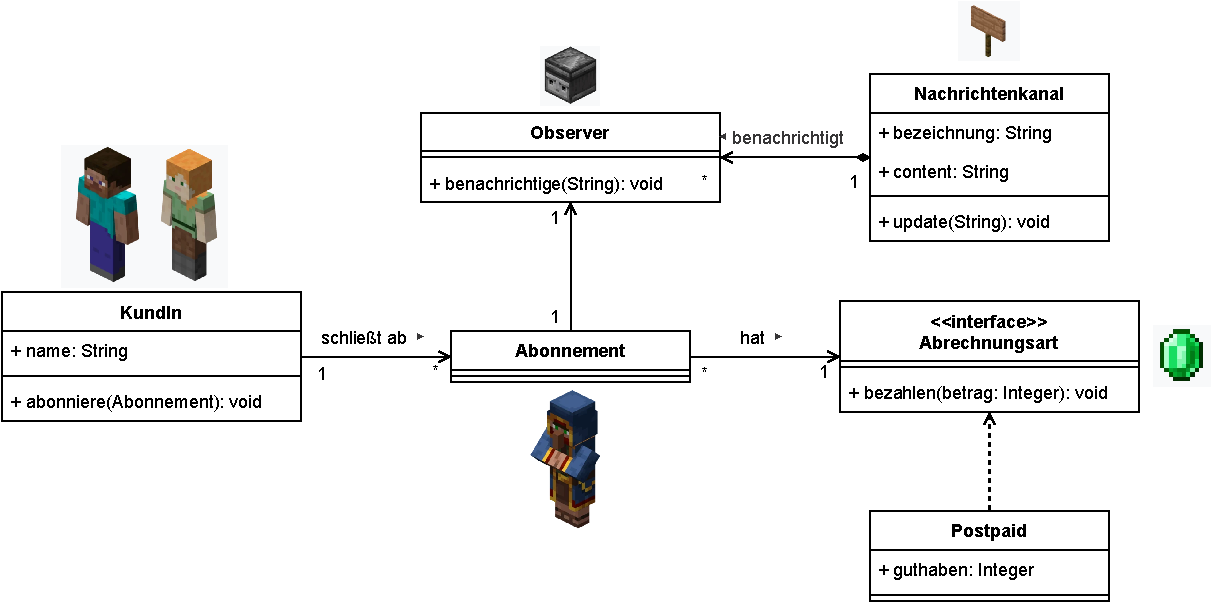
\includegraphics[width=\textwidth]{swt_wende_tim_h08_class_diagram_pre.pdf}
                \caption{\texttt{class\_diagram\_pre}}
            \end{figure}

            \newpage
            Da diese offensichtlich von dem fertigen Code abweicht, hier nochmal eine aktualisierte Version:
            \begin{figure}[ht]
                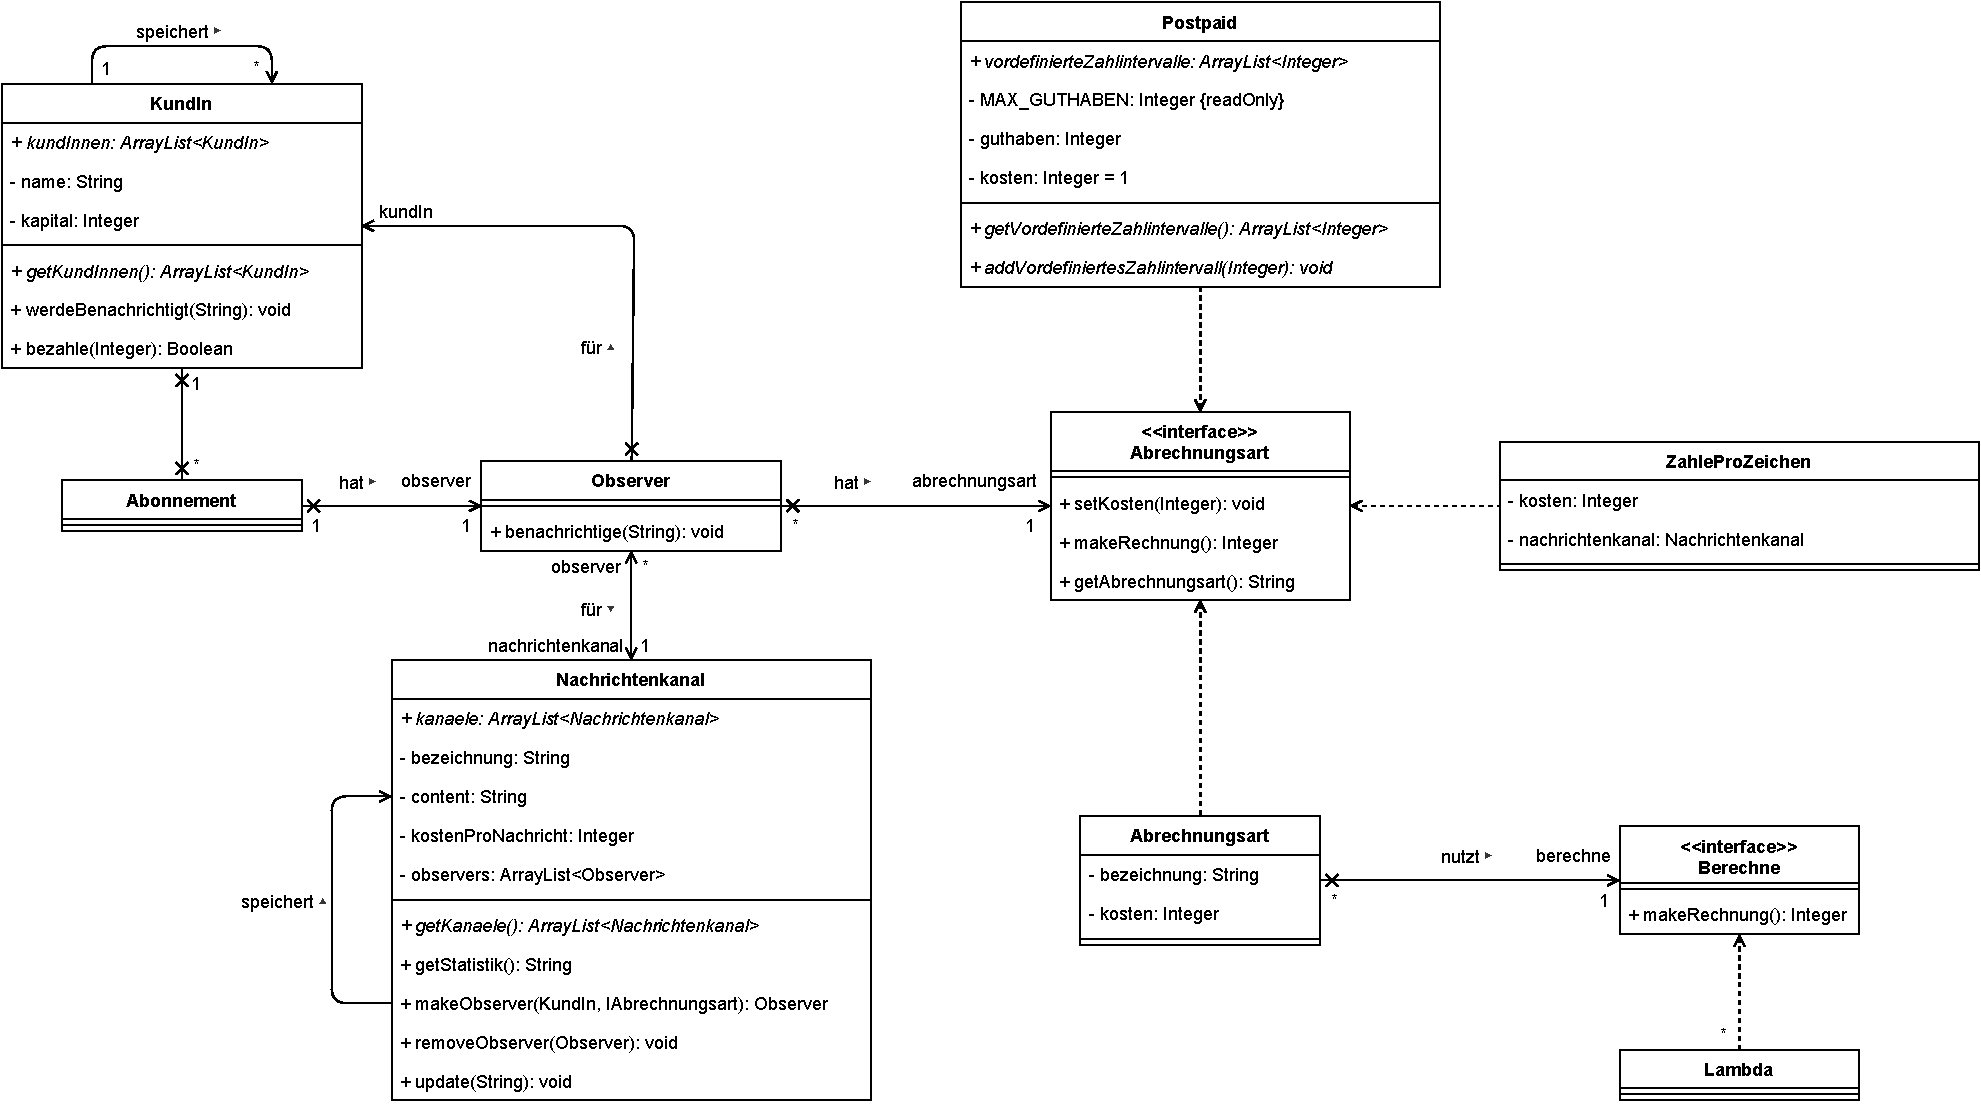
\includegraphics[width=\textwidth]{swt_wende_tim_h08_class_diagram_post.pdf}
                \caption{\texttt{class\_diagram\_post}}
            \end{figure}

            Diese unterscheiden sich nicht großartig voneinander, die zweite Version, welche nach der ersten Iteration revisiev erstellt wurde, ist jedoch ausführlicher und weiß genauer, welche Datentypen genutzt wurden.

            \begin{itemize}
                \item Observer-Observable-Pattern
                    
                    Als Observer dient die Klasse \gqq{Observer}\\
                    Als Observable dient die Klasse \gqq{Nachrichtenkanal}

                    Nachrichtenkanal speichert alle zu sich gehörenden Observer und ruft deren \texttt{benachrichtige}-Methode auf, sollte sich der Content ändern.
                    Dies geschieht weder automatisch via Trigger noch sonst irgendwie sinnvoll.
                    Nach Rücksprache stellte sich heraus, dass der Vorgang, wie hier zu sehen, gewollt ist.
                \newpage
                \item Strategy-Pattern
                
                    Vorab: man hat 2 Möglichkeiten Abrechnungsarten hinzuzufügen
                
                    \begin{figure}[ht]
                        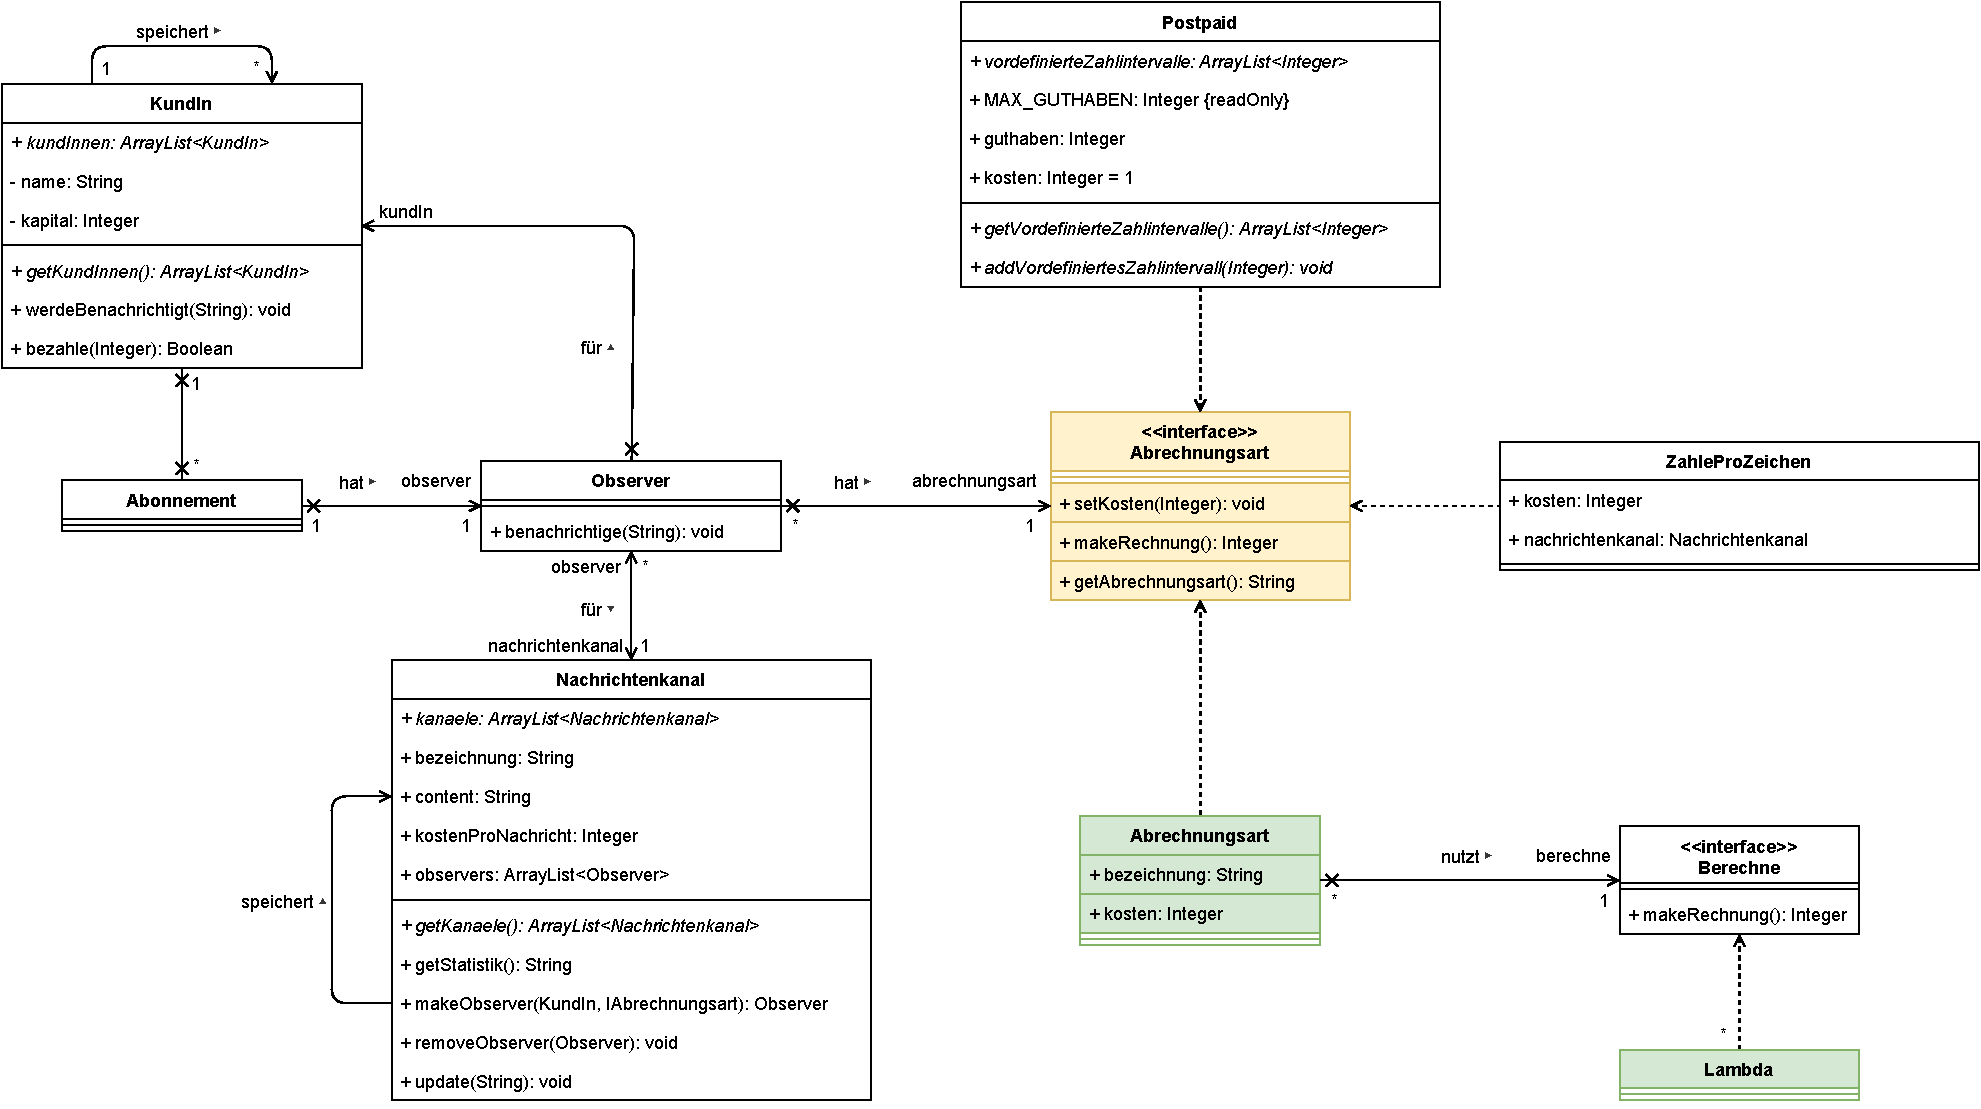
\includegraphics[width=\textwidth]{swt_wende_tim_h08_class_diagram_options.pdf}
                        \caption{\texttt{class\_diagram\_options}}
                    \end{figure}
                
                    \begin{enumerate}[label=\arabic*.]
                        \item Man erstellt eine \textcolor{orange}{Klasse} und implementiert \gqq{IAbrechnungsart}

                        \begin{minted}{java}
public class ZahleJedeNachricht implements IAbrechnungsart {
    int kosten;

    public void setKosten(int kosten){
        this.kosten = kosten;
    }

    public int makeRechnung(){
        return -1 * betrag;
    }

    public String getAbrechnungsart(){
        return "Zahle jede Nachricht";
    }
}
                        \end{minted}

                        \item Man erstellt ein \textcolor{green}{Objekt} der Klasse \gqq{Abrechnungsart} mit einer \texttt{Bezeichnung} und einem \texttt{Lambda Ausdruck}, welcher als Parameter und return einen \underline{int} erhält/ zurückgibt.

                            \begin{minted}{java}
new Abrechnungsart("Zahle jede Nachricht", betrag -> -1 * betrag);
                            \end{minted}
                    \end{enumerate}

                    Für \gqq{einfache} Abrechnungsarten sei die zweite Methode zu bevorzugen.
            \end{itemize}
            
        \newpage
        \item Geben Sie dann \texttt{Implementierungen} aller Klassen an.
        Beachten Sie, dass für versandte Nachrichten eine Abrechnung erfolgen muss.
        Binden Sie den Nutzungsdialog (siehe Main.java und Beispiel-Output) mit ein.
        Mit ihm kann man neue Nachrichten und Kunden anlegen.
        Außerdem kann der Kunden Nachrichtenkanäle mit einer auswählbaren Abrechnungsart wählen und Informationen über alle Nachrichtenkanäle zusammen mit den angefallenen Abokosten anzeigen.
        Natürlich kann man auch die Nachrichteninhalte eines Nachrichtenkanals verändern. Der Nutzungsdialog kann nach einigen Schritten wie folgt aussehen, Eingaben sind umrandet (Die Datei Main.java sollte entsprechend ergänzt werden). 

        Schauen wir uns dazu erstmal den gegebenen sowie meinen Output an:

        \begin{figure}[ht]
            \centering
            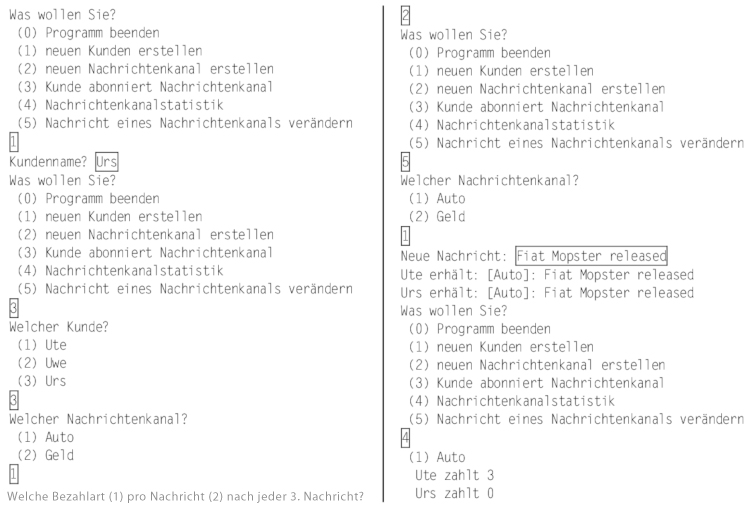
\includegraphics[width=0.65\textwidth]{class_diagram.jpg}
            \caption{\texttt{class\_diagram\_01}}
        \end{figure}

        \begin{figure}[ht]
            \centering
            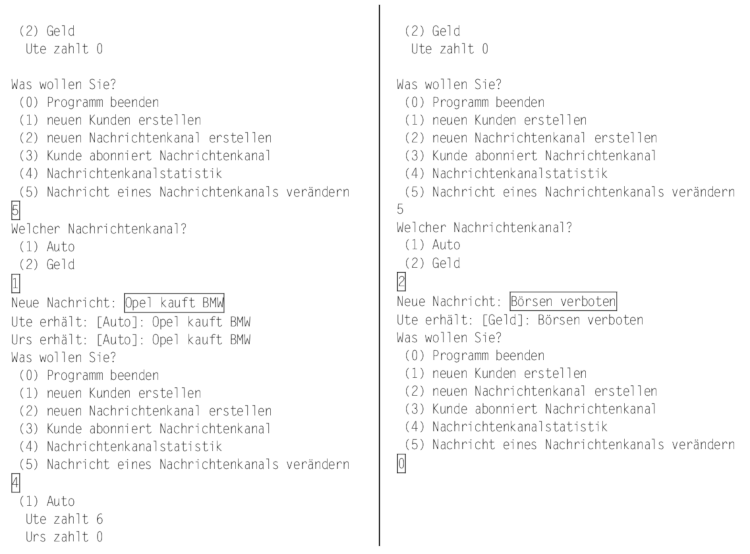
\includegraphics[width=0.65\textwidth]{class_diagram.png}
            \caption{\texttt{class\_diagram\_02}}
        \end{figure}

        \newpage
        \VerbatimInput{out.txt}

        \newpage
        Zusätzlich der Output von ein paar automatisch getesteten Klassen bzw. erstellten Objekten:

        \VerbatimInput{simulation.txt}

        \newpage
        Diese wurden von meiner Testklasse erstellt:
        \inputminted{java}{Test.java}

        Schauen wir uns zuerst die kleine Hilfsklasse \texttt{Abonnement} an:\\
        Sollte \texttt{getStatistik} den bereits bezahlten Betrag ausgeben, kann man dies hier implementieren.
        Ansonsten kann die Klasse im Grunde auch gelöscht werden.
        \inputminted{java}{Abonnement.java}

        \newpage
        Schauen wir uns nun \texttt{KundIn} an:
        \inputminted{java}{KundIn.java}

        \newpage
        Von hier aus gehen wir weiter zu \texttt{Observer}:
        \inputminted{java}{Observer.java}

        \newpage
        Und nun zu Nachrichtenkanal:
        \inputminted{java}{Nachrichtenkanal.java}

        Dieser benötigt ein Objekt des Intefaces mit der statischen Klasse IAbrechnungsart:
        \inputminted{java}{IAbrechnungsart.java}

        \newpage
        Implementierte Klassen sind beispielsweise:
        \inputminted{java}{Postpaid.java}
        Sowie:
        \inputminted{java}{ZahleProZeichen.java}

        \newpage
        Des weiteren existiert die Klasse \texttt{Abrechnungsart}, welche \texttt{IAbrechnungsart} Lambda-fähig macht:
        \inputminted{java}{Abrechnungsart.java}

        Diese benötigt:
        \inputminted{java}{IBerechne.java}
    \end{enumerate}
\end{document}